\chapter{Regression Summary}
\section{Likelihood Emulation As Standard Regression}\label{sec:emulation_as_regression}
% \chapter{Likelihood Emulation}
% menziona metodi likelihood-free tipo abc? cfr astroabc

% Noi comunque qui vogliamo valutare esattamente i valori della likelihood; magari a meno di normalizzazione uno può comunque fare così per campionare dalla stessa...

% \section{Regression Recap}
% imparare un mapping fra dati (modello, loss, algoritmi vari tipo GD), under overfitting con bias variance tradeoff, interpretabilità
As said in the introduction a cosmological emulator is simply a substitute for the exact mapping between cosmological parameters and quantities like power spectra; we already remarked several times that the relation between these quantities is of paramount importance to cosmological likelihood functions. Even though this situation is specific to cosmology the way we address it is not unique: determining an approximation of the function mapping a set into another is an example of a \emph{regression problem}, which is quite common in modern science. For this reason it pays off to review the theory behind regression, focusing in particular on some common regression models; this discussion will pave the way for \textsc{CosmoLIME}, which in a sense is nothing more than a glorified, automated regressor.

An important remark is that, as we saw in the previous chapter, it is often advantageous to learn to replicate the relation between cosmological parameters and power spectra, i.e. ``indirect'' likelihood representations. This is important, because it means that instead of learning to emulate a \emph{distribution} we can focus on the conceptually easier task of emulating a \emph{function}.\footnote{One may argue that the distinction between the two is negligible, especially in the case of Gaussian likelihoods, which in principle are simple functions of mean and covariance; and yet this distinction is more important than it may seem. For example not all distributions admit a (simple) functional representation; e.g. Gaussian distributions may require unfeasible matrix inversions. More in general if the likelihood is non-Gaussian or does not admit an exact functional form (as in the case of a realistic CMB likelihood), or if only data sampled from the likelihood are available (instead of direct likelihood values), the problem becomes significantly more involved; in order to learn the likelihood we may need e.g. MCMC techniques, etc., instead of the simple mapping learning performed in functional regression.
By emulating only the ``easy'' functional (i.e. deterministic) part of the likelihood we can focus on efficiently isolating the theoretical dependence of the likelihood on cosmological parameters, leaving the rest to the complete parameter inference.}

Having understood why our general goal is emulating a function $f$ we remark that this can be done by sampling the function (i.e. obtaining a certain number of $\{x_n, f(x_n)\}$ pairs) and learning from them the shape of $f$. 
In general $f$ is unknown and this must be done by e.g. experimentally measure these pairs; in the case of cosmological emulation $f$ is available and can be used to \emph{compute} an arbitrary number of exact $\{x_n, f(x_n)\}$ pairs (indeed the goal is not to discover an unknown function, but rather to accelerate the evaluation of a known one).
The fact that we can compute as many noise-free $f(x)$ samples as we want is a peculiar and unique property of the \emph{emulation task}, which really sets it apart from the generic regression problem (where the data are in fixed number and potentially noisy); we will discuss this in more detail later on in section \ref{subsec:simulating_data}. For now it suffices to remark that once the dataset has been obtained (either by simulation, as in the emulation task, or by ``experiment'', as in the general regression setting) these tasks converge into the same problem: learning (an approximation of) the function that maps a vector space into another. In practice this means that, except for the peculiar way in which the data are obtained, \emph{the emulation task is just another regression problem}; for this reason the fitting techniques to be used are the same general supervised learning methods used to predict continuous variables. Therefore it makes sense to review some basic results from regression theory; discussing these is the purpose of this chapter. The techniques and properties of the problem presented in the following sections represent the solution to the second part of the emulation task (i.e. approximating $f$ using $\{x_n, f(x_n)\}$ pairs), and therefore will provide us with a crucial \textsc{CosmoLIME} piece; as already anticipated the results needed to deal with the first part (i.e. actually obtaining data via simulation) will be discussed in section \ref{subsec:simulating_data}. For now let us assume the problem of obtaining valid data samples has been already solved, and that therefore we only need to figure out how to find a good approximation of $f$.

\section{A Primer On Regression}
\subsection{Problem Setup}
% mapping, modello, loss, algoritmi
Imagine we have a dataset $\mathcal{D} = \{\mathcal{X}, \mathcal{Y}\}$ containing an input dataset $\mathcal{X} = \{x_i\}_{i=1}^N$ and an output one $\mathcal{Y} = \{y_j\}_{i=1}^N$, where all $x_i$ and $y_i$ values are either real numbers or vectors of real numbers. We assume there exists a function $f$ relating the two datasets - namely, $f$ maps each of the $x_i$ into the corresponding $y_i$:
\begin{equation*}
    f(x_i) = y_i
\end{equation*}
In the context of e.g. simulating power spectra $f$ is known but expensive to compute; the theory about regression is more general, though, and in most machine learning applications $f$ is actually unknown. The theory even allows for $f$ to be not partially stochastic; for example a common occurrence is that some additive noise is assumed to be corrupting $f$'s output. For all these reasons the fact that in cosmology we actually know the exact form of $f$ is irrelevant: the regression procedure is the same - namely, it learns the patterns in the training data in order to construct a suitable approximation of $f$. The idea is that we would like to find another function, $\hat{f}$, such that its outputs approximate those of $f$ as closely as possible:
\begin{equation*}
    \hat{f}(x_i) = \hat{y}_i \approx y_i \quad \forall i = 1, \dots, n
\end{equation*}
In order to ensure that the above condition is satisfied a similarity measure between $\hat{y}_i$ and $y_i$ is needed; such a measure is commonly called \emph{error function}. Thanks to an error function it becomes possible to assign a score to $\hat{f}$, which can be used to choose $\hat{f}$ between several candidates. In practice this can be done by computing the error as the \emph{ensemble average over all possible data realizations} of a certain \emph{loss function} $\ell(f, \hat{f})$, which measures how ``wrong'' each prediction $\hat{f}(x)$ is compared to the true value $f(x)$:
\begin{equation*}
    L_\mathcal{D}(f, \hat{f}) = \expval{\ell(f, \hat{f})}_\mathcal{D}
\end{equation*}
The error function is defined over all possible data realizations, because we care about the similarity between the two functions $f$ and $\hat{f}$, not just between their outputs on this particular dataset (prediction close to true values over $\mathcal{D}$ do not necessarily imply the same performance over another dataset $\mathcal{D}'$). Since in general we don't have access to the data generation distribution we can only estimate the true error using the \emph{training error}, i.e. the sample mean computed using the training data at our disposal; but this is just an estimate of a quantity that cannot be computed, which may or may not be accurate (see the next section). In general the subscript $\mathcal{D}$ as a reminder that this is the loss estimated over our particular dataset.

Having defined the error function we now have to choose a particular loss function.
A common approach to do this relies on using a metric or a norm; this is reasonable if we assume that similarity between function can be expressed as closeness in some space according to some definition of distance.

There exists several loss functions designed according to this idea; the most common one is probably the \emph{Euclidean} loss, also called $\ell_2$ loss; the error associated to this function is simply the Euclidean norm (squared) of the vector difference between the true and predicted values, divided by the number of samples:\footnote{We replaced the $\mathcal{D}$ subscript because this is just the estimate of the true error over a single realization $D$ instead of the ensemble average computed over the infinitely many possible datasets. $L_D$ is the training error over dataset $D$; $L_\mathcal{D}$ is the true error averaged over all possible dataset instances.}
\begin{equation*}
    L_D(f, \hat{f}) = \frac{1}{N} \norm{y - \hat{y}}_2^2 = \frac{1}{N}\sum_{i=1}^N \abs{y_i - \hat{y}_i}^2 = \frac{1}{N}\sum_{i=1}^N \abs{f(x_i) - \hat{f}(x_i)}^2
\end{equation*}
This error is common because it represents the average residual, i.e. the average Euclidean distance between the true and predicted values. For this reason another the above is also commonly called the \emph{mean squared error} (MSE), since the difference between true and predicted values represents the error in the prediction.
Of course there are other ways of defining similarity or distance between $f$ and $\hat{f}$; this is the most popular because it has a nice interpretation (average residual, i.e. mean squared error) and other remarkable mathematical properties (for example it allows for an analytical solution of the gradient descent algorithm in the case of linear predictors).
Ideally a perfect predictor has an error equal to zero, because $\hat{y}_i = y_i$ exactly and for all $i$; in practice we have to settle for values that are ``close enough'' to zero, according to an arbitrary definition of ``close enough''.

In general defining an error $L_D(f, \hat{f})$ is important because it allows one to establish the basic algorithm shared by all regression techniques. In order to perform regression in practice we restrict our attention to the functions belonging to a specific set of functions $\mathcal{F}$, often called the \emph{hypothesis class}; for example one can choose the set of linear predictors, which are the models computing the output as a linear combination of the input features. Once this is done we can pick the member of $\mathcal{F}$ that minimizes the error $L_D(f, \hat{f})$, and that will be our $\hat{f}$ predictor of choice.\footnote{The reason why one must restrict themselves to only a specific form for $\hat{f}$ candidate is twofold: clearly in practice it would be impossible to test an infinite number of functional dependences, but there are also theoretical limitations (as shown in \cite{understanding_ml} unless the hypothesis set $\mathcal{F}$ is restricted in some way overfitting becomes unavoidable).} A popular algorithm that implements these ideas in practice is \emph{stochastic gradient descent}: assuming $\hat{f}_w$ has a fixed form but depends on a set of parameters $w$ the algorithm walks around $w$ space settling in one of the minima of the training error $L_D(f, \hat{f}_w)$ - which is now a function of the $w$ vector.

Putting everything together the steps to perform regression i.e. to find $\hat{f}$ approximating $f$ are the following:
\begin{enumerate}
    \item acquire a dataset $\mathcal{D} = \{\mathcal{X}, \mathcal{Y}\} = \{(x_i, y_i)\}_{i=1}^N$;
    \item pick a training error function $L_D(f, \hat{f})$ and a family of models i.e. a set of functions $\mathcal{F}$ to whom $\hat{f}$ must belong;
    \item choose the member of $\mathcal{F}$ that minimizes the training error according to some minimization algorithm (e.g. gradient descent).
\end{enumerate}
This procedure is quite simple, conceptually speaking; as a consequence dealing with regression is one of the simplest problems in machine learning. Still there are several nuances that deserve attention, as they make the task of obtaining a suitable $\hat{f}$ less trivial than it may seem; we discuss some of these in the following sections.

\subsection{The Bias-Variance Trade-off}
% discussione generale di approximation error ecc di understanding + la forma esplicita con la varianza nei termini di ISLP: la varianza fra se riallenassi lo stesso modello con questi dati e altri, eccetera
% se memorizza troppo bene il training set non riesce a generalizzare ai sample non visti del test set...
% figure dell'esempio di regressione polinomiale di understanding e magari un plot dei due errori durante un training/al crescere della complessità del modello: underfitting, compromesso, overfitting

% nota di contestualizzazione: abbiamo visto come il test ultimo di accuracy sia la gara di inferenze (cosmopower), ma prima ancora di arrivarci possono sorgere problematiche di overfitting...
% nota di introduzione: nella sezione precedente sembra che basti avere una loss bassa, ma bisogna stare attenti: overfitting eccetera

\subsubsection{The Bias-Complexity Trede-off}
In the previous section we stated that, when training a regressor, one must always choose between functions belonging to a restricted family (e.g. the set of linear functions, etc.); this is counterintuitive, as one would expect that picking $\hat{f}$ from the set of all possible functions would allow the training algorithm to perform better.

It can be shown that this is not true due to the \emph{no free lunch theorem}, i.e. the fact that \emph{there is no universal learner}. In practice this means that any algorithm trying to learn a predictor picked from an unrestricted set of functions will always fail, i.e. a competing algorithm selecting from a restricted family of functions will always perform better.

Therefore it is mandatory to restrict the set of potential learners; this can be done e.g. by using prior knowledge to decide which type of function seems reasonable for the problem at hand.
This restriction makes learning possible, but introduces the \emph{bias-complexity trade-off}, i.e. the idea that we must choose a set $\mathcal{F}$ that is neither too rich nor too poor. A general discussion of this trade-off can be found in \cite{understanding_ml}; for our purposes it suffices to understand how this trade-off is related to the concepts of \emph{under/overfitting} and the specific form it takes in the case of the regression task.

\subsubsection{Overfitting And Underfitting}
Let us reproduce an example from \cite{understanding_ml} to explain the concepts of overfitting and underfitting.

Imagine we are trying to learn to predict the data in the following figure:
\begin{figure}[H]
    \centering
    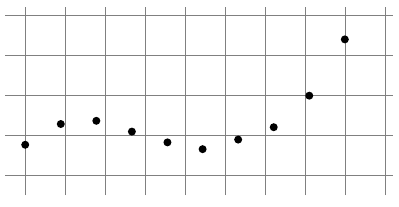
\includegraphics[width=0.6\textwidth]{img/polinomio_dati.png}
    \caption{Data to learn from with a polynomial regression model.}
\end{figure}
If we try to use a polynomial regression model with degrees 2, 3 or 10 we may find functions like these:
\begin{figure}[H]
    \centering
    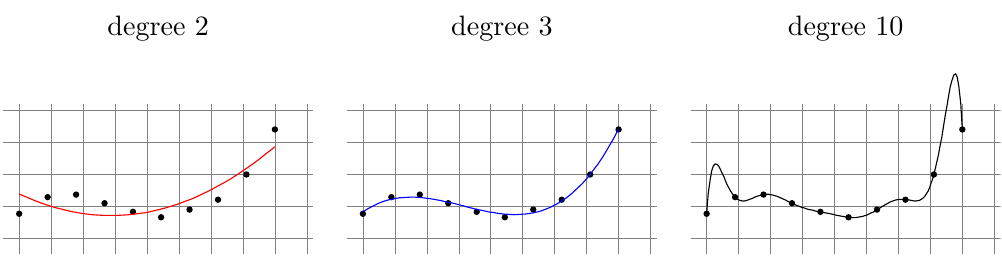
\includegraphics[width=1.0\textwidth]{img/polinomio_fit.png}
    \caption{Polynomial fits of degrees 2, 3 and 10.}
\end{figure}
Increasing the degree $d$ of the polynomial increases the model's complexity, and with it its capability of fitting the data; indeed we see that with larger values of $d$ the polynomial can be made to more precisely go through the black points, which is reflected on the fact that increasing $d$ decreases the training error i.e. the error evaluated on the training dataset.

Let us define a \emph{test set}, i.e. a second dataset containing samples not seen during the training phase; we can compute the \emph{test error} and compare it to the training error as functions of the degree $d$.
\begin{figure}[H]
    \centering
    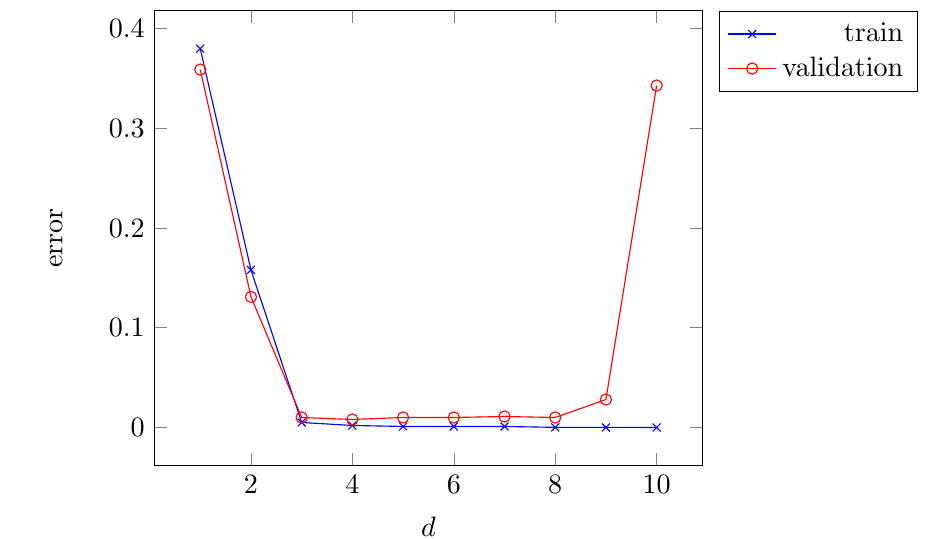
\includegraphics[width=1.0\textwidth]{img/polinomio_curve.png}
    \caption{Model selection curves for the polynomial regression example (for now the distinction between test and validation set is irrelevant).}
\end{figure}
We notice that the simplest models (low $d$) have high training \emph{and} test error; then as $d$ grows they both decrease, up to a point where the test error rises again. Let us explain why this happens.

Simple models (i.e. models chosen with a stronger bias on $\mathcal{F}$) cannot fit arbitrary data arbitrary well; for this reason they tend to have relatively high errors on any dataset. At the same time since we optimize them using a stronger bias their performance does not depend significantly on the data used to test it, therefore this has the advantage that the training error paints an accurate picture. This scenario is called \emph{underfitting}, i.e. the model does not learn enough from the dataset but its performance is reliable on arbitrary datasets.

The opposite happens for complex models: they can always fit arbitrary data much better, but at the cost of learning too well the training dataset. This can lead to models e.g. simply memorizing the random noise inside the data, instead of learning the true patterns inside it. Therefore even though their training error is very low the test one is high, which means that this model simply memorize the training data and fail to successfully generalize to new samples. This scenario is called \emph{overfitting}, i.e. the model learns the patterns inside the data too well and can end up learning random noise or just memorizing the training data.

Notice in particular that an underfitting model generalizes well in the sense that it has the same bad performance over all datasets, while an overfitting model generalizes poorly in the sense that it has good performance on the training data and terrible accuracy on every other datasets.
In both cases we observe that the test error is the truly universal indicator of a model's performance, while the training error can be potentially unreliable and deceiving in the case of overfitting.
This is a general property: it can be shown that \emph{the test error is a better estimate of the true error compared to the training error} \cite{understanding_ml}.

As we can see from the previous figure models that sit in between avoid both of these bad scenarios: in particular their predictions are accurate enough on both seen and unseen data, i.e. they generalize well to new datasets; this means they learn the correct patterns.

In order to ensure the model used has the right amount of complexity a common practice in machine learning is to define a test set as above, i.e. set aside some samples and use them to see how well the model generalizes to new data; as we will see this procedure is automatically employed inside \textsc{CosmoLIME}.

\subsubsection{Bias-Variance Trade-off in Regression tasks}
In the specific problem of regression we can derive a quantitative expression that captures the essence of this trade-off.

Let us assume as usual that the available data has been generated according to $y=f(x)+\varepsilon$, where $f$ is a deterministic unknown function and $\varepsilon$ is random noise; then the point of regression is learning a function $\hat{f}$ that can approximate $f$.

Let us assume that we are using the mean squared error; this means that the training error over a dataset $D$ is given by
\begin{equation*}
    L_D(y, \hat{y}) = \frac{1}{N} \sum_{n=1}^N\abs{f(x_i)-\hat{f}(x_i)}^2
\end{equation*}
This is just an estimate of the true error obtained by approximating the ensemble average with the sample average; the true error is instead computed by averaging over all possible data realizations. Using the $\ell_2$ loss we can write:
\begin{equation*}
    L_\mathcal{D}(f, \hat{f}) = \expval{\left(f(x_0)-\hat{f}(x_0) \right)^2}_\mathcal{D}
\end{equation*}
where $x_0$ is any point. 
As said before this quantity cannot be computed exactly, only estimated using the test error. 
To better understand how this quantity reacts to the model's complexity we can use a general decomposition (see \cite{islp} for proof):
\begin{equation}
\label{eq:bias_variance_tradeoff}
    \expval{\left(f(x_0)-\hat{f}(x_0) \right)^2}_\mathcal{D} = \mathrm{Var}\left(\hat{f}(x_0)\right) + \left[\mathrm{Bias}\left(\hat{f}(x_0)\right)\right]^2 + \mathrm{Var}(\varepsilon)
\end{equation}
We already know that the quantity on the left hand side is the ensemble average of the loss over any possible point, i.e. the expected test error; let us focus on the right hand side.

The last term is simply the variance of the noise. Notice that all the terms on the right are always positive, and that $\mathrm{Var}(\varepsilon)$ does not depend on the model; this means that even if we could set to zero the first two (e.g. by finding the perfect $\hat{f}$) there would still be an irremovable source of error due to noise. This makes sense; intuitively we expect that we can never go below the noise, i.e. we can never perform perfect predictions because the true value of $y$ is in part random.

The remaining two terms depend on the choice of $\hat{f}$, and we can easily show they have opposite effects.
The first term is the \emph{variance of the statistical learning method}, i.e. the amount by which $\hat{f}$ would change if we used a different training dataset. This term grows with the model's complexity: as we saw before complex model fit the data so accurately that small changes in the training data can result in large changes in $\hat{f}$.
Due to this we learn that a) this term measures the model's complexity, and b) that we should avoid having too much complexity because through the variance term it causes the expected test error to grow.
The other term is the model's \emph{bias}, i.e. the error introduced by approximating $f$ with an $\hat{f}$ that is too simple. This term decreases as the model's complexity increases: as we saw in the  polynomial example models that are too simple are not flexible enough to accurately learn to reproduce \emph{any} data, which means that a high bias will cause an increase in the expected test error.

We recover once again the trade-off between too much bias and too much complexity. Increasing or decreasing the model's complexity can both lead to worse overall performance; careful tuning is needed to ensure we find a good compromise.
As discussed in the previous section this can be done in practice by computing the test error (which provides a more accurate estimate of the true error) and plotting learning curves; now we have a more sound theoretical explanation for why these tools can help identify overfitting and underfitting, as well as an explanations for why these happen in the first place.

\subsection{Accuracy Metrics: $L_2$ vs $R^2$}\label{subsec:accuracy_metrics}
% L2 ed R2; distinto da loss ad es. $\chi^2$ (cfr loss prof)
% cosmopower paper: il test ultimo è la gara delle inferenze; faticoso ma risolve il problema di "quanto piccolo deve essere il test error perché ci sentiamo a posto?" Mezzo compromesso = R^2

% cfr https://scikit-learn.org/stable/modules/model_evaluation.html#dummy-estimators : r2 si basa sul predictor costante, uno può fare paragoni con dummy predictors più generali. In generale rivedi quella pagina https://scikit-learn.org/stable/modules/model_evaluation.html per prendere spunto per tutta la sezione

% comunque conta di più l'inferenza
In the previous section we discussed that statistically speaking the test error provides a better estimate of the true error. Let us assume that we have computed a test error for a given regression task and that it indeed represents an unbiased estimate of the ideal error; the problem we have then to face is how to interpret the obtained value.
Said in another way: how can we decide when the test error is low enough that the model can be considered successful?

By definition the test error depends on the choice of the loss, which means the numerical values it can take change depending on arbitrary choices; this means that some ways to measure model performance may be more interpretable than others. Indeed a common machine learning practice is to compute a selection of several \emph{accuracy metrics}, whose numerical values may lend themselves to easier interpretations.

An example of this is given by the relation between the $L_2$ and the $R^2$ metrics, which we now discuss.
The $L_2$ error on a dataset $D = \{x_i, y_i\}$ for a predictor $\hat{f}$ is given by
\begin{equation*}
    \frac{1}{N}\sum_{i=1}^N \abs{y_i-\hat{y}_i}^2 = \frac{1}{N}\sum_{i=1}^N \abs{y_i-\hat{f}(x_i)}^2
\end{equation*}
A perfect predictor would achieve $\hat{f}(x_i) = y_i \ \forall i$, which would cause the $L_2$ loss to become equal to zero. As the predictor gets farther and farther away from the perfect predictor the $L_2$ error grows; for an arbitrarily bad model the $L_2$ error can be arbitrarily large.
This means that the lower the $L_2$ error, the better; but how can we decide when the error is low enough? For example: is 0.01 low enough? What about 0.001?
Clearly the answers to these questions depend on the problem at hand and on the user's accuracy requirements; still we can compute an alternative metric, which is equivalent to the $L_2$ error but normalized in such a way that is easier to understand.

\begin{equation}
    R^2 = 1 - \frac{\sum_{i=1}^N \left(y_i-\hat{f}(x_i)\right)^2}{\sum_{i=1}^N (y_i-\bar{y})^2}
\end{equation}
where $\bar{y}$ is the sample mean of the $y_i$ values; this quantity is called \emph{coefficient of determination}.
We notice that the fraction on the left hand side is simply the ratio between the MSE and the mean square deviation of the $y_i$ values from their mean; said in another way we are comparing the average residual of the predicted values with a quantity that is proportional to the variance of the $y_i$ values; this helps normalizing the MSE score.
Indeed this fraction is useful because it can be used to determine not only if the MSE is small enough (i.e. close enough to zero), but actually if it is small enough \emph{compared to the dataset's intrinsic variability}. For example an MSE equal to 0.1 is quite good if on average the variation in allowed $y_i$ values is of order 100; the fraction on the right hand side precisely quantifies this point.

By subtracting this fraction from 1 we gain an even more interpretable normalization. Indeed we notice that a perfect predictor has $R^2=1$, since it will always satisfy $y_i=\hat{f}(x_i)$; a predictor that instead constantly outputs the mean $\bar{y}$ has $R^2=0$.
Due to this we can use the $R^2$ metric as a more interpretable counterpart of the $L_2$ error; in particular a value of $R^2$ close to 1 means the model is close to the perfect predictor (at least on the provided data), whereas a model with $R^2<0$ performs worse than a model constantly predicting the dataset's average. More generally $R^2$ can be used to measure how close the current model is to these two extreme cases; for this reason it represents a good candidate for an accuracy metric.

In general defining metrics that compare the model to ``dummy predictors'' (e.g. models that output constant values, random numbers, etc.) is a common technique in machine learning. We argue that $R^2$ represents the best compromise between simplicity and usefulness; for this reason it is the default metric inside \textsc{CosmoLIME}.
Of course arbitrary metrics are allowed, but since we find the $R^2$ coefficient to be good enough we are content with discussing and recommending just this accuracy metric.


% \subsection{Interpretability}
% discussione generale; l'esempio di linear regression (gradiente = coefficienti) e generalizzazione a NAM perché mi piace VENGONO DOPO - o meglio: qui puoi fare l'introduzione contenente effettivamente l'esempio di linear regression e generalizzazione con funzioni arbitrarie di ogni input tenuto separato, menzionando che se come f(x_i) usi reti neurali ottieni il modello che descrivi meglio sotto (sotto puoi citare il paper, parlare delle interazioni di ordine superiore, e così via per allungare il brodo)

\section{Common Machine Learning Regression Models}\label{sec:ml_models}
% i 3 modelli più sensati da descrivere (vedi sotto). Inoltre meglio fare una descrizione molto veloce, molto en passant, senza troppe formule, tanto per dire cosa faccia ciascuno di questi modelli - e cosa offra, tipo la non sensibilità degli alberi da normalizzazione, un buon compromesso fra velocità e accuracy specie con xgboost e simili, eccetera.

We now briefly review some common machine learning models for the regression task. As we will see in the next \textsc{CosmoLIME} supports arbitrary models, but still recommends tree-based models or neural networks. The reason for this is that we find tree-based models to offer a nice balance between training speed and accuracy, whereas neural network are one of the most powerful models commonly used in practice; in our tests they both fared favourably.
Therefore it makes sense to summarize some results about these models; in particular we base the following discussion on \cite{islp}, \cite{understanding_ml}, \cite{ml_probabilistic_perspective}.
Many other powerful and interesting models such as Gaussian process-based regressor are popular choices for cosmological emulation; since a complete discussion would be too long we choose to focus on just two families of models as an example of how regression predictors actually work in practice.

\subsection{Tree-based models}
% vantaggi e svantaggi, tipo indipendenza dal rescaling di media e varianza o minmax, velocità di learning, somiglianza con il ragionamento umano, interpretabilità persa con metodi basati o meno su bagging ecc ma che permettono più potenza e meno tendenza a overfitting

% su questo e altro cita understanding machine learning e introduction to statistical learning, i paper originali tipo quello di xgboost

% puoi citare anche probabilistic perspective


 %\subsubsection{Decision Trees}
% adatta https://tex.stackexchange.com/questions/289642/how-to-draw-a-proper-decision-tree al caso di una regressione, ad esempio scrivendo prima a formule una serie di disuguaglianze nested (tipo con la notazione delle funzioni per casi). Va bene mettere direttamente prima quello come esempio elementare nel caso di classification/variabili categoriche (utile riguardo al discorso "modello simile al ragionamento umano", eccetera)

% modo in cui cattura le interazioni fra variabili


 %\subsubsection{Random Forests}
% https://tikz.net/random-forest/ ma non era bootstrapping al posto di bagging? Capire e in caso adattare. La stessa figura con label diversi penso si possa usare nel caso del boosting a seguire

% introduzione stile understanding di weak learners potenziati? In quel senso si ha il "boosting" generico, non necessariamente gradient boosting ecc.

 %\subsubsection{Gradient Boosting}
% magari non serve una figura, visto che somiglierebbe a quella precedente; quindi magari basta discutere a parole il discorso del gradiente

% \subsubsection{Explainable Boosting Machines}
% interpretabilità recuperabile con albero di sintesi...
% ma anche explainable boosting machines di microsoft? Fa figo forse

\emph{Tree-based models} are a vast class of models that has seen a resurgence in popularity with the development of powerful packages like \texttt{xgboost}; due to how cheaply they allow us to obtain surprisingly accurate predictions (along with other benefits such as interpretability) they are a welcome addiction to \textsc{CosmoLIME}'s recommended models. Indeed it often happens in practice that a tree-based model can outperform more complex ones with just a fraction of the time and data needed to achieve convergence; even in situations where more complex models are needed it often makes sense to first try with tree-based models, given how cheap training them is.
In particular in our simple tests no other family of models came as close to achieving solid performance in such a short amount of time and with as little data; hence it only makes sense to briefly touch on their properties.

The simplest type of tree-based model is the \emph{decision tree}, which can be used both in classification and in regression tasks; a graphical representation of such a model is given in the following figure.

\begin{figure}[H]
    \centering
    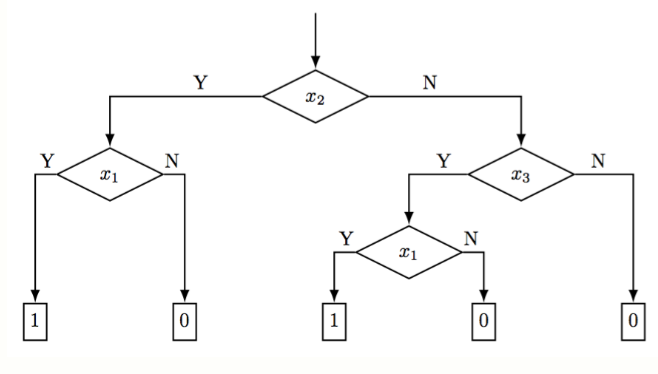
\includegraphics[width=0.9\textwidth]{img/decision_tree.png}
    \caption{An example of a decision tree.}
    \label{fig:decision_tree}
\end{figure}

In order to output a result a decision tree asks a series of nested binary questions on the features i.e. components of the input. For example in figure \ref{fig:decision_tree} the tree first asks a question about the $x_2$ component; depending on the yes/no binary answer the tree splits into two \emph{branches}, that further split and so on until we are left with \emph{leaves} collecting all possible output predictions depending on the input.
This ensures decision tree models are easy to interpret; in particular we can exactly see how they came to a particular conclusion, because the path they followed is ``transparent''; the same cannot be said for black-box models such as neural network. Interpretability is especially useful as a diagnostic tool, because in the case of a training failure we can exactly see what the model has learned wrong.

In the case of regression the binary questions asked at each tree split are inequalities about the input features; for example a tree may choose different paths depending on whether variable $x_2$ is less than 3, and so on.
Since a decision tree can only use a finite number of inequalities what it does is to essentially \emph{bin the input and output values}: input features in the same interval will be mapped to the same output. Geometrically this is equivalent to stating that \emph{decision trees divide the input space into rectangular decision regions}; if a certain point has coordinates individually inside certain intervals its output will be that of the corresponding rectangle.

Decision trees are cheap to train due to the commonly used greedy algorithm (see e.g. \cite{islp}), and also offer relatively good accuracy as long as the problem at hand is not too hard to learn - with the added benefit of interpretability, as mentioned above. Another nice feature of decision trees is that they are \emph{insensitive to scale} \cite{islp}, i.e. feature standardization has no effect on them. The reason for this is trivial: if a certain tree computes whether e.g. $x_2<3$ or not and we scale the input features by 2 then the same tree will be produced by the training algorithm, just with $x_2'<6$ as the new test equality.


The main disadvantage of decision trees is that they are not very powerful in the sense that they can struggle with very complex problems; a common approach to improve their power is to consider an \emph{ensemble} of trees, since a collection of weak learners can be shown to be equivalent to a single strong learner (see \cite{understanding_ml}), a principle informally called \emph{wisdom of the crowds}.

A popular type of tree-based ensemble model is the \emph{random forest} model. A random forest obtains its prediction by consulting a large number of simple trees (either by computing the mean in the regression task or by majority vote in the classification task); these trees are individually trained by presenting them with \emph{bootstrapped versions} of the original training dataset. What this essentially means is that starting with the training dataset several other datasets are created, each with a random selection of the original samples with repetition. Due to this each member in the forest is presented with a different dataset, and can therefore \emph{specialize} on different patterns contained in the original dataset. 
The price to pay for this improvement in performance is that the model is no longer easily interpretable and takes longer to train - both consequences of the increased complexity.

Another common type of ensemble model is \emph{gradient boosting}, recently popularized by the excellent \texttt{xgboost} framework. Once again several trees are trained to compute the final prediction, but this time they are all trained on the original dataset. What changes is how the prediction is computed; in particular the first tree learns a crude approximation of the target, then the second tree learns the \emph{residual} of the first trees's prediction (i.e. the difference with the true value), and so on. In this way the final approximation is given by this recursive sum single tree outputs. This significantly increases the model's power because each tree can specialize on a different resolution, i.e. focus on different orders of magnitudes; we will revisit this idea under a more general light in the next section.
Another advantage of this approach is that the learning task can be reframed in a way that allows the use of \emph{gradient descent}-based algorithms; software packages like \texttt{xgboost} take advantage of this to build approximate histogram-based internal data representations that can significantly speed up training with only a small decrease in final accuracy.
Just as with random forests this model's increased complexity makes it both more powerful and more expensive compared to simple decision trees, as well as less transparent; the trade-off between these competing pursuits should be carefully taken into account by the user when choosing which model to use.












\subsection{Neural Networks}\label{subsec:nn}
\begin{comment}
flessibili ma pesanti e pertanto lente (tanti parametri), schizzinose (molti dati richiesti e preprocessing delicato), training potenzialmente instabile (gradient dying, explosion, ecc), no interpretabilità
% \subsubsection{Feedforward Fully Connected NNs}
le reti neurali sono sensibili alla scala dei parametri perché prendono combinazioni lineari degli stessi, mettendo quindi tutto sullo stesso piano in termini numerici. Ad esempio una rete che prenda due input features, una variabile fra 1000 e 2000 e l'altra variabile fra 1 e 2, sarà praticamente insensibile alla seconda feature anche se magari fisicamente una variazione da 1 a 2 è in realtà estremamente significativa e dovrebbe portare a predizioni molto diverse. Allora per compensare la rete deve imparare ad usare pesi molto sbilanciati per compensare (ad esempio 0,1 e 100), ma questo può portare a instabilità numeriche (gradiente che impazzisce), quindi meglio tagliare la testa al toro e fare noi una normalizzazione perfettamente e facilmente invertibile in modo da avere solo valori (sia features che pesi) dell'ordine dell'unità. Ovviamente siccome il problema è l'instabilità numerica del training (in linea di principio basta compensare coi pesi e tutto si sistema) e quest'ultima non si manifesta sempre/sempre allo stesso modo non sempre standardizzare aiuta, ma va comunque tenuto in conto come opzione da almeno considerare. Nota: questo problema non si verifica con gli alberi perché ogni feature ha i suoi range, le disuguaglianze usate per decidere il percorso da prendere tengono distinte le features. Chiaramente questa questione è legata al fatto che siano presenti o meno somme e più in generale che i valori numerici di ciascuna feature contribuiscano allo stesso modo alla predizione, infatti un problema analogo si può avere con modelli più semplici tipo la regressione lineare

% https://tikz.net/neural_networks/ copia prima la figura con x e y e poi quella con le formule alla fine (riferendola ad un layer generico nel mezzo, così puoi giustificare la notazione "a" al posto di x e y)

https://stats.stackexchange.com/questions/7757/data-normalization-and-standardization-in-neural-networks
discutere qui questa teoria per poi ritirarla in ballo nel preprocessing di cosmolime sotto

modo in cui cattura le interazioni fra variabili
\end{comment}

\emph{Neural networks} are a vast family of models that exploded in popularity in the last few decades due to the exponential increase regarding affordable computational power. A fair discussion of neural networks would be impossibly long; for this reason we are content with quickly explaining how they work.

\begin{figure}[H]
    \centering
    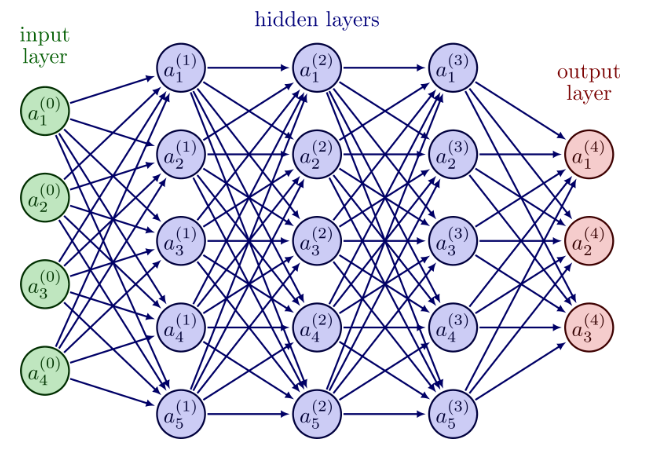
\includegraphics[width=0.9\textwidth]{img/neural_network.png}
    \caption{A graphical representation of a simple feedforward fully connected neural network.}
    \label{fig:neural_network}
\end{figure}
The most basic type of neural network is called the \emph{feedforward fully connected network}; a graphical representation of this type of architecture is given in figure \ref{fig:neural_network}.
This kind of network consists of a series of layers, each containing a certain number of elementary units called \emph{neurons}. Each neuron is connected to every other neuron in both the previous and the next layers; a weight is assigned to each connection.
In order for the network to perform predictions the input vector is first disassembled into its components, which are then fed in the first \emph{input layer}; these values are then propagated forward until the \emph{output layer}, where the vector prediction can be collected. 
To propagate the values from the input to the output layer each neuron takes all the values returned by the previous one, then computes a linear combination of these numbers using the weights associated to the corresponding connection; finally a nonlinear function is applied (called the \emph{activation function}), and the result is then passed to the next layer.

Neural networks are popular because they are very powerful models: thanks to the large number of parameters and the nonlinear activations they can learn complex patterns with impressive accuracy. The price to pay for this power is that neural networks are very hard to train and even harder to train \emph{successfully}; this is unavoidable considering their high intrinsic complexity, which is also the source of their ability to perform impressive feats.

For example due to the large number of trainable parameters (i.e. the connection weights) neural networks are complex models, which makes them prone to overfitting; to prevent this strong regularization penalties often have to be implemented, which significantly slows down training as the modification of weights becomes more conservative.
The large number of weights that must be trained and the complicated technique that is often used to do it (i.e. \emph{backpropagation}) also mean that training is computationally expensive; not only that, but neural networks are ``hungry'' models, i.e. compared to simpler ones typically require larger datasets to achieve comparable accuracy. These unavoidable issues were the reason why until recently using neural networks was not really feasible in practice.

Another delicate fact that further complicates training is that neural networks can become numerically unstable; for example when training with SGD and backpropagation the gradient can ``die'' for certain choices of the architecture, i.e. the network may become unable to update its weights.
Another numerical issue is that neural networks internally sum values that may be defined over different orders of magnitude; in this case careful feature normalization/standardization is needed to ensure that the network does not lose resolution or internal numerical stability.

These are just some example that show how high the price of using neural networks can be; and yet with the right approach training them successfully can definitively be done, resulting in a predictor with potentially stunning accuracy, for example much better than other popular models.




\begin{comment}
\subsubsection{Neural Additive Models}
menzionare brevemente perché fa figo? Paper di google; interazioni fra variabili comunque aggiungibili ma che ha senso tenere sotto controllo, ad es. permettendo solo coppie e visualizzando l'interazione in questione su un piano...


\subsection{Other Regressors}
penso basti menzionare a lista qualche altro modello, tipo i gaussian processes, magari le svm con i kernel, eccetera, tanto per ma senza perderci troppo tempo.

OPPURE: visto che a sto punto mi sono solleticato l'interesse da solo riciclo parte della teoria scritta sopra per spiegare come si usano i GP nella regressione, così si può fare il discorso interessante sullo smoothing dovuto al kernel e sul posterior predictive, eccetera. Alla fine non è così importante essere esaustivi con i modelli, o anche con i dettagli sui GP stessi.
bonus point: così sto esaminando solo i modelli più sensati (alberi perché mi piacciono e sono sottovalutati, ad esempio non so quanti conoscano xgboost come fuoriclasse in regressione fuori dalla community di data science, reti neurali e GP perché sono i modelli più usati negli emulatori cosmologici)
\end{comment}

% Comunque alla fine della fiera per dati quadrati i modelli ad albero offrono un ottimo compromesso fra velocità e accuracy essendo poco schizzinosi (sia per esperienza con cosmolime sia in generale tipo ad es con xgboost), al massimo uno si spara una rete neurale e buonanotte; per queste ragioni i modelli raccomandati con cosmolime sono solo quelli, e tuttavia il software è in grado di utilizzare classi arbitrarie ad esempio dotate di metodi train e predict (facoltativamente score)


%\subsection{Precision Machine Learning} % tecnicamente non è un regressor a sé ma un modo per potenziarne uno preesistente, almeno nel caso del fit dei residui... però non mi va di fare una sezione a se stante per una cosina così breve, al massimo se riesco ad unirla ad altro per fare una sezione "altro", boh! Pensaci su
\section{\textit{Precision Machine Learning} Regime}\label{sec:precision_ml}
\begin{comment}
introduzione simpatica a questa sezione: mentre finora in questo capitolo abbiamo evidenziato le somiglianze fra il nostro problema specifico (emulazione cosmologica) e un sacco di altri problemi in ML (proprio una categoria più generale) adesso discutiamo una particolarità del nostro problema, qualcosa di raro: il fatto di potere avere dati infiniti e perfetti, quando di solito il dataset è fissato (raccolto una tantum e basta) e contiene del rumore ineliminabile del tutto E IL FATTO DI AVERE FUNZIONI REGOLARI| dati infiniti relativi ad una prediction stocastica al massimo ti permettono di predire perfettamente le probabilità di osservare qualcosa, non esattamente l'output, stile QM; nel nostro caso le funzioni da emulare sono perfettamente deterministiche e simulate (da questi due punti segue l'assenza di rumore) e REGOLARI (questo ci permette in linea di principio di emularle senza troppa fatica). Questo ci porta nel regime di precision learning: spiegare cosa voglia dire e menzionare alcune tecniche per far scendere la loss fino a questi livelli disumani. Non mi va di discutere più di tanto tutte le tecniche del paper, al quale rimanderei, anche per la discussione teorica su come si comportino i vari modelli; penso basti menzionare gli algoritmi di ottimizzazione del secondo ordine, eccetera. Invece vorrei discutere nel dettaglio il fit dei residui, perché è una cosa molto semplice e molto simpatica, oltre che molto facile da implementare in pratica (magari provo al volo a fare un fit di questo tipo negli esempi più difficili del prof)

facciamo così: se non è più semplicemente il posto dove mettere il fit dei residui si merita la sua sezione a parte.

A parte riferire i risultati del paper ha senso usare questo spazio come posto dove discutere più nel dettaglio il discorso di dati infiniti e puliti in quanto simulati - e questo è il motivo per cui il regime PML è pertinente, oltre ad essere il presupposto di design fondamentale su cui si basa cosmolime (perché altrimenti una emulazione soddisfacente potrebbe non essere possibile, perché altrimenti non avrebbe senso dare la possibilità di definire un target arbitrario, eccetera)


cita il paper, spiega più nel dettaglio come la combo dati infiniti + dati senza rumore (likelihood regolare e che possiamo valutare a nostro piacimento) permetta di scendere a valori di loss bassi potenzialmente fino alla machine precision...
Tecniche varie per raggiungere questo risultato: penso la più interessante sia il fit dei residui, ma comunque è bene dare un'altra occhiata al paper

vedendolo di sfuggita: interessanti le discussioni sui vari regimi, come scalino diversi modelli, quando sia possibile il regime di precision ml eccetera.
\end{comment}
Up until this section we mostly discussed the points shared between the emulation task and the generic regression task, such as the techniques to find an approximation of a function given a certain dataset, etc.; we now want to focus on the most important difference between the two - namely, the number and quality of available data.

As discussed in section \ref{sec:emulation_as_regression} the emulation task is unique because we have access to $f$, i.e. the exact regression target; this means we can compute as many exact samples as we want to assemble the training dataset. In the standard regression this is not possible; the dataset is collected only once, and noise may ruin its quality. Let us discuss this difference more in detail.

\begin{itemize}
    \item The first consequence of knowing $f$ is that \emph{the dataset is noise-free}; this means that the $\mathrm{Var}(\varepsilon)$ term in equation \eqref{eq:bias_variance_tradeoff} is zero.
    \item The second consequence of knowing $f$ is that \emph{the dataset can have an arbitrarily large size}, i.e. by computing new samples as needed. As discussed several times we can only estimate the model's true error, e.g. by using the test error; this is equivalent to estimating the ensemble average with the sample average. Ensuring these two are as close as possible is important because otherwise we are led to overfitting, i.e. we mistakenly believe the model's performance is great but when presented with new data it performs poorly. Since the sample average converges to the ensemble one as the number of samples grows by simulating new points we can get an arbitrarily accurate estimate of the true error, i.e. of the model's performance irrespective of any dataset it may see in the future. Having such an accurate estimate of the true error therefore allows the model to steer towards the perfect predictor during training.
    \item In the particular case of cosmological power spectra emulators it can be shown that the target functions are usually smooth with respect to their input parameters (see for example sec. \ref{subsec:figure_cmb_power_spectrum}); this means that a perfect predictor actually exists, and therefore that a powerful enough machine learning model can become arbitrarily close to this predictor.
\end{itemize}
By combining these points we obtain that \emph{in the emulation task the model's error can become arbitrarily close to zero}. This follows from the fact that the fundamental limit to the model's error due to noise has been removed, and from the fact that by arbitrarily increasing the size of the dataset we can get optimize an arbitrarily good estimate of the true error; this is also due to the fact that the simple properties of $f$ allow for the existence of the perfect predictor.

This situation where it becomes possible to achieve arbitrarily low error values is defined as \emph{Precision Machine Learning Regime} in \cite{precision_ml}. In this study the authors analyze the implications of this regime, especially focusing on how different models (e.g. neural networks, polynomial functions) behave under these conditions.
An interesting aspect of \cite{precision_ml} is that the authors discuss several techniques that can be used to actually reach an error arbitrarily close to zero; this is not trivial, because the precision machine learning regime only guarantees that zero error is \emph{possible}, not that it is necessarily reached in practice.
In \cite{precision_ml} several tools are analyzed, such as second order methods to improve the standard stochastic gradient descent algorithm. A particularly powerful technique they present is \emph{sequential residual fitting}; this idea is as simple as it is powerful, and therefore deserves a brief discussion.
Suppose that instead of training a single predictor $\hat{f}$ we train two models $\hat{f}_1$ and $\hat{f}_2$ sequentially according to this rule: first train $\hat{f}_1$ to fit $f$, then train $\hat{f}_2$ to fit the residual $(f-\hat{f}_1)/c$, where $c\ll 1$ normalizes the residual to unity to ensure numerical stability. The two models can then be combined into a single predictor $\hat{f}(x) = \hat{f}_1(x)+c\hat{f}_2(x)$.
This can lead to significant performance improvements because it allows the final predictor to be sensitive to variations over different orders of magnitude, i.e. $\hat{f}$ has the same high resolution w.r.t. both large and small variations of the input parameters. Increasing the model's resolution over multiple scales can significantly improve the model's performance, as discussed in \cite{precision_ml}; this technique is also trivial to implement, and therefore recommended in \textsc{CosmoLIME} to achieve the arbitrarily low errors made possible by the peculiar properties of the emulation task.

To recap: the fact that in the emulation task the target function $f$ is known means that an arbitrarily high number of noise-free samples may be obtained; from this it follows that the emulation task is an example of the \emph{precision machine learning regime}, i.e. it allows to in principle obtain arbitrarily low errors.\footnote{The fact that we can generate perfect samples with generosity is one of \textsc{CosmoLIME}'s core design principles, as we will discuss in the next chapter.}
Techniques such as those explained in \cite{precision_ml} may be used to actually achieve this perfect result in practice; \emph{sequential residual fitting} is particularly nice, because it is powerful but trivial to implement.